\newcommand{\Title}{Little Robot} 
\title{\Title}

\documentclass[a4paper]{article}
\usepackage{geometry}
\geometry{a4paper,tmargin=25mm,bmargin=35mm,lmargin=20mm,rmargin=20mm,footskip=5mm}
\usepackage[utf8x]{inputenc}
\usepackage{fontspec}
\usepackage{graphicx}
\usepackage{subcaption}
\usepackage{capt-of}
\usepackage{lastpage}
\usepackage[ngerman]{babel}
\usepackage[colorlinks=true,linkcolor=black,urlcolor=black]{hyperref}
\usepackage[headsepline,footsepline]{scrlayer-scrpage}
\usepackage{multirow}
\usepackage{listings}            
\usepackage{makeidx}

\usepackage{xcolor,soul}
\usepackage{colortbl} % Farbige Tabellen

\usepackage{longtable}

\pagestyle{scrheadings}
\clearscrheadfoot

\definecolor{LightGray}{rgb}{0.9,0.9,0.9}
\newcommand{\CItoprowcolor}{\rowcolor{LightGray}}

%%Head
\ihead{{\textbf{\large \Title}}}
\ohead{\raisebox{0.1\totalheight}{
\includegraphics[width=0.15\textwidth]{../pictures/wak-lab-LOGO.png}}}

%%Foot
\cfoot{\pagemark}
\ofoot{\today}


\begin{document}
\maketitle
%\tableofcontents
\begin{center}
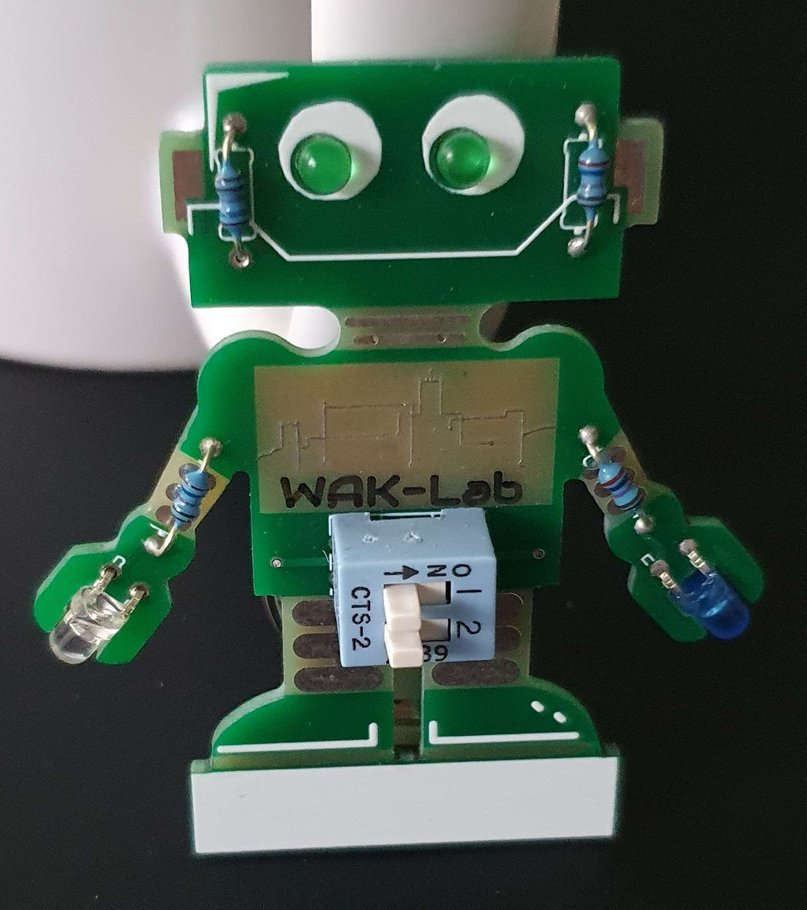
\includegraphics[height=8cm]{../pictures/RoboAus.jpg}
\ \\
Design: Martin Hildebrandt\\
licensed CC BY\\
\ \\
Logo: By Dorothea Wendt\\
licensed CC BY-ND\\
\end{center}
\newpage
\section{Einleitung}
Der Bausatz ist als kleine Lötübung für einen einfachen Stromkreis mit  4 LEDs, 2 Schalter 4 Widerständen und eine Knopfzelle CR2032.\\
\ \\
\begin{minipage}[t]{\textwidth}
  \centering
  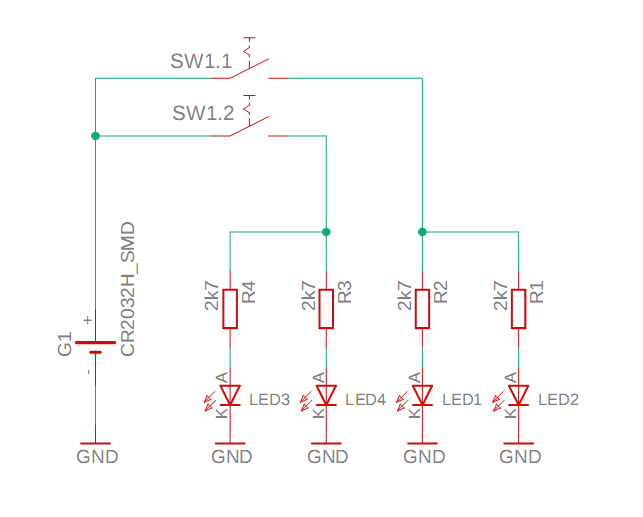
\includegraphics[width=0.5\textwidth]{../pictures/Schematic}
  \captionof{figure}{Schaltplan}
  \label{img:Schematic}
\end{minipage}
\ \\

\subsection{Kurz etwas zum Löten}
Beim Löten stellen wir eine feste Verbindung aus Metall her. Dazu wird der Lötkolben auf ca. 350$^{\circ}$C eingestellt. Die Bauteile werden beim Löten sehr hei\ss \ und können nicht mit dem Finger gehalten werden (Verbrennungsgefahr). Die Lötspitze darf auch nie den Tisch berühren, dass hinterlässt hässliche Brandflecken. Der Lötkolben ist immer sicher zu lagern und das Anschlusskabel und die Steckdose sicher verlegt sein (Stolpergefahr).\\
Zunächst wird das Bauteil eingefädelt. Das Beinchen vom Bauteil kann etwas nach au\ss en gebogen werden, damit es fixiert ist. Dann mit dem Lötkolben Pad und Beinchen aufheizen und dann etwas Zinn von der gegenüber liegen den Seite heranführen und aufschmelzen. Nach etwas 1-2 Sekunden sollte genug Zinn an der Verbindung sein. Die Zeit kann stark variieren je nach dem wie viel Wärme von Bauteil oder Pad aufgenommen wird.\\
\ \\
Zum Löten benötigen Wir:
\begin{itemize}
  \item     Den Bausatz
  \item     einen Lötkolben
  \item     etwas Lötzinn
  \item     einen Seitenschneider
  \item     eine feuerfeste Unterlage
  \item     optional eine Flachzange
\end{itemize}

\section{Aufbau}
\begin{minipage}[t]{\textwidth}
  \centering
  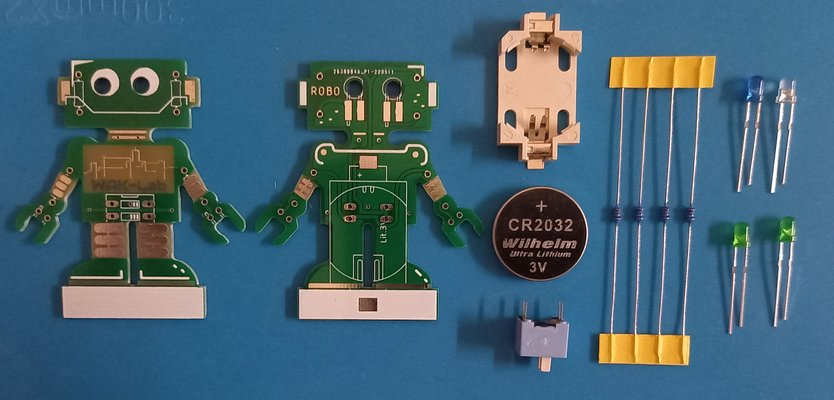
\includegraphics[width=0.9\textwidth]{../pictures/Parts.jpg}
  \captionof{figure}{Bauteile}
  \label{img:Bauteile}
\end{minipage}
\ \\
\begin{minipage}[t]{0.33\textwidth}
  \centering
  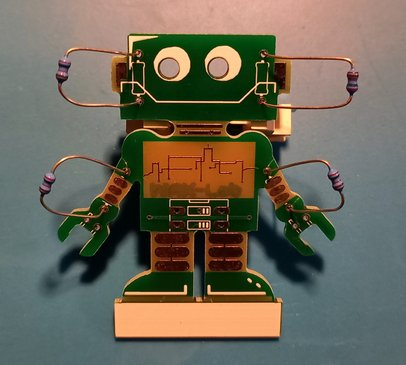
\includegraphics[height=4cm]{../pictures/Resistor1.jpg}
  \captionof{figure}{Widerstände}
  \label{img:Resistor1}
  \end{minipage}
\begin{minipage}[t]{0.33\textwidth}
  \centering
  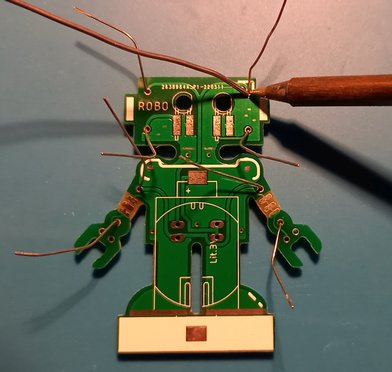
\includegraphics[height=4cm]{../pictures/Resistor2.jpg}
  \captionof{figure}{Widerstände}
  \label{img:Resistor2}
\end{minipage}
\begin{minipage}[t]{0.33\textwidth}
  \centering
  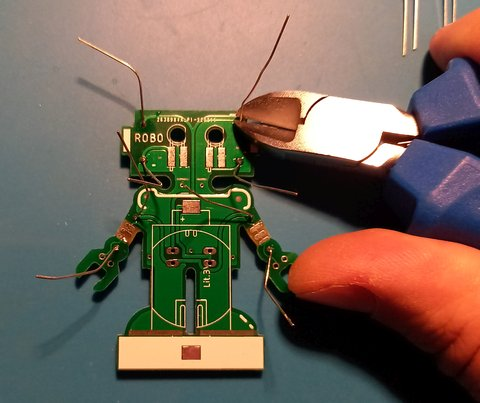
\includegraphics[height=4cm]{../pictures/Resistor3.jpg}
  \captionof{figure}{Widerstände}
  \label{img:Resistor3}
\end{minipage}
\ \\
\begin{minipage}[t]{0.33\textwidth}
  \centering
  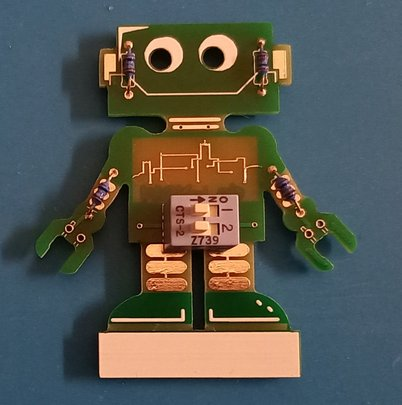
\includegraphics[height=4cm]{../pictures/Switch1.jpg}
  \captionof{figure}{Schalter}
  \label{img:Resistor1}
  \end{minipage}
\begin{minipage}[t]{0.33\textwidth}
  \centering
  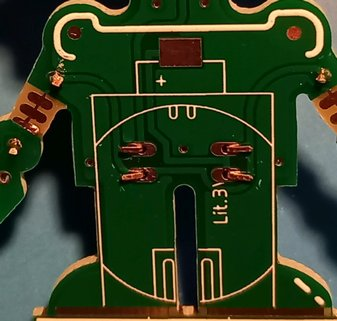
\includegraphics[height=4cm]{../pictures/Switch2.jpg}
  \captionof{figure}{Schalter}
  \label{img:Switch2}
\end{minipage}
\begin{minipage}[t]{0.33\textwidth}
  \centering
  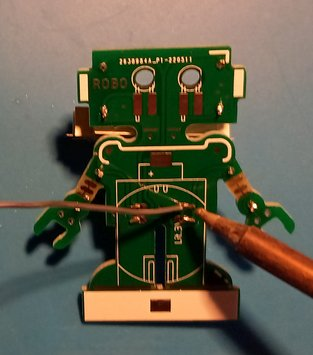
\includegraphics[height=4cm]{../pictures/Switch3.jpg}
  \captionof{figure}{Schalter}
  \label{img:Switch3}
\end{minipage}
\ \\
\begin{minipage}[t]{0.33\textwidth}
  \centering
  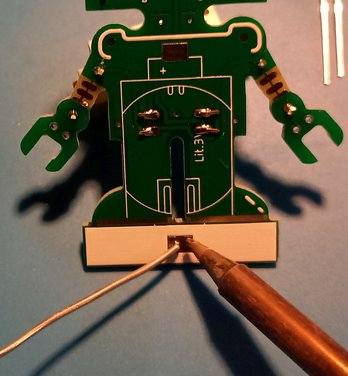
\includegraphics[height=4cm]{../pictures/Bat1.jpg}
  \captionof{figure}{Batteriehalter}
  \label{img:Bat1}
  \end{minipage}
\begin{minipage}[t]{0.33\textwidth}
  \centering
  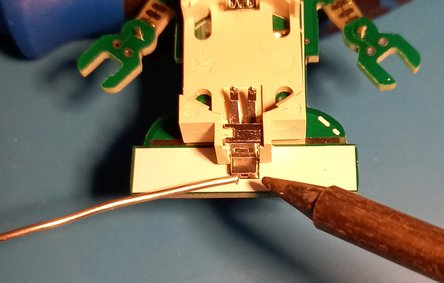
\includegraphics[height=4cm]{../pictures/Bat2.jpg}
  \captionof{figure}{Batteriehalter}
  \label{img:Bat2}
\end{minipage}
\begin{minipage}[t]{0.33\textwidth}
  \centering
  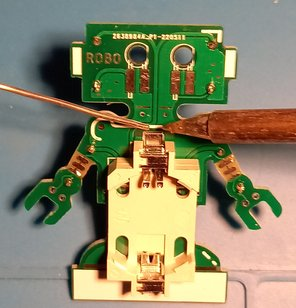
\includegraphics[height=4cm]{../pictures/Bat3.jpg}
  \captionof{figure}{Batteriehalter}
  \label{img:Bat3}
\end{minipage}
\ \\
\begin{minipage}[t]{0.33\textwidth}
  \centering
  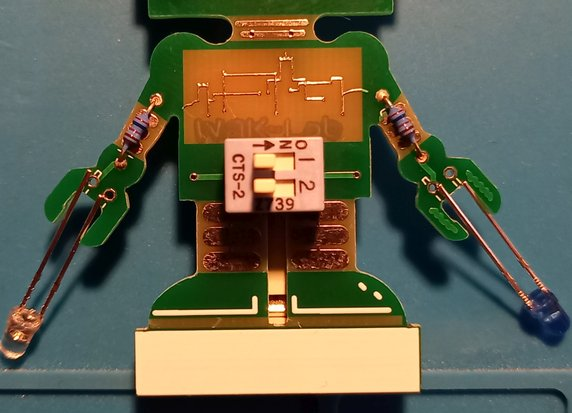
\includegraphics[height=3.5cm]{../pictures/LED1.jpg}
  \captionof{figure}{LED}
  \label{img:LED1}
  \end{minipage}
\begin{minipage}[t]{0.33\textwidth}
  \centering
  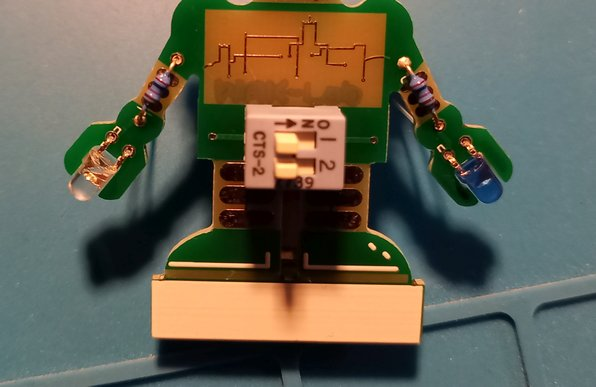
\includegraphics[height=3.5cm]{../pictures/LED2.jpg}
  \captionof{figure}{LED}
  \label{img:LED2}
\end{minipage}
\begin{minipage}[t]{0.33\textwidth}
  \centering
  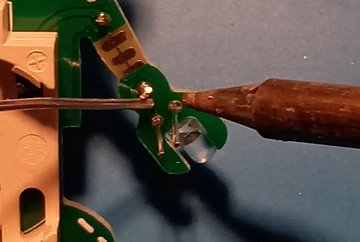
\includegraphics[height=3.5cm]{../pictures/LED3.jpg}
  \captionof{figure}{LED}
  \label{img:LED3}
\end{minipage}
\ \\
\begin{minipage}[t]{0.33\textwidth}
  \centering
  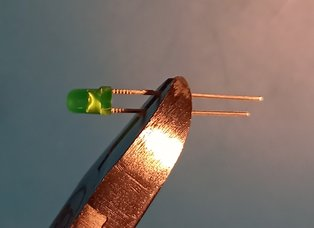
\includegraphics[height=3.5cm]{../pictures/LED4.jpg}
  \captionof{figure}{LED}
  \label{img:LED4}
  \end{minipage}
\begin{minipage}[t]{0.33\textwidth}
  \centering
  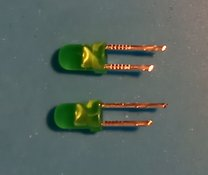
\includegraphics[height=3.5cm]{../pictures/LED5.jpg}
  \captionof{figure}{LED}
  \label{img:LED5}
\end{minipage}
\begin{minipage}[t]{0.33\textwidth}
  \centering
  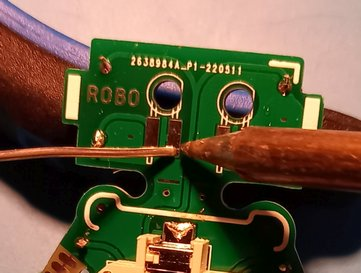
\includegraphics[height=3.5cm]{../pictures/LED6.jpg}
  \captionof{figure}{LED}
  \label{img:LED6}
\end{minipage}
\ \\
\begin{minipage}[t]{0.33\textwidth}
  \centering
  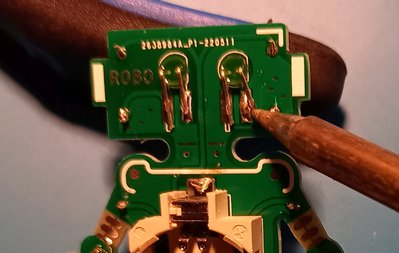
\includegraphics[height=3.5cm]{../pictures/LED7.jpg}
  \captionof{figure}{LED}
  \label{img:LED7}
  \end{minipage}
\begin{minipage}[t]{0.33\textwidth}
  \centering
  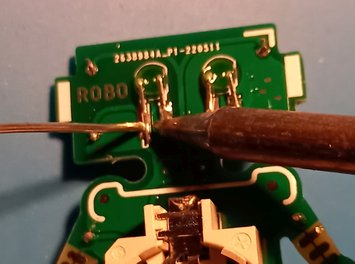
\includegraphics[height=3.5cm]{../pictures/LED8.jpg}
  \captionof{figure}{LED}
  \label{img:LED8}
\end{minipage}
\ \\
\begin{minipage}[t]{0.33\textwidth}
  \centering
  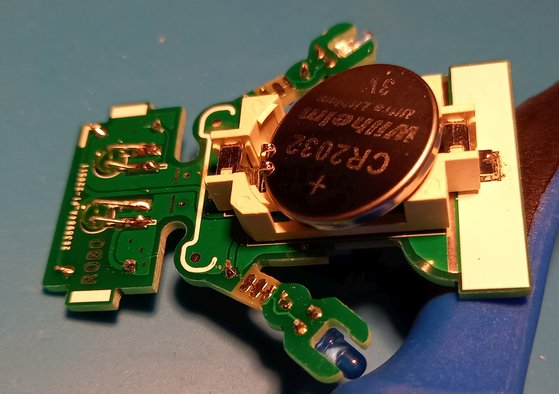
\includegraphics[height=3.5cm]{../pictures/Bat4.jpg}
  \captionof{figure}{LED}
  \label{img:Bat4}
  \end{minipage}
\begin{minipage}[t]{0.33\textwidth}
  \centering
  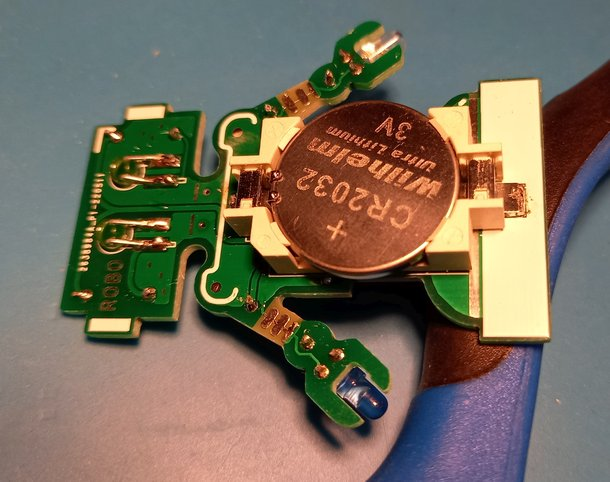
\includegraphics[height=3.5cm]{../pictures/Bat5.jpg}
  \captionof{figure}{LED}
  \label{img:Bat5}
\end{minipage}
\begin{minipage}[t]{0.33\textwidth}
  \centering
  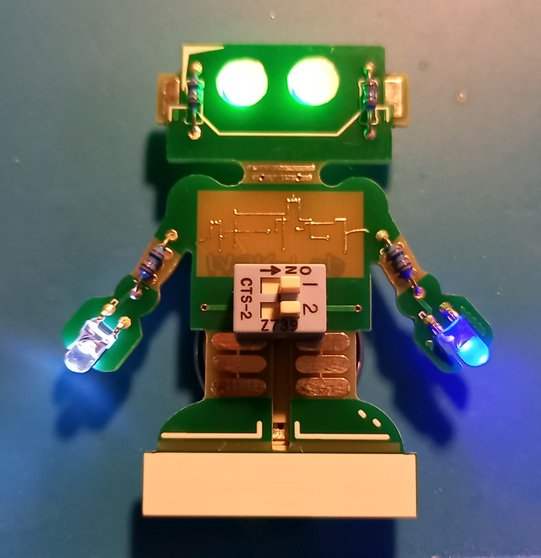
\includegraphics[height=3.5cm]{../pictures/Ready.jpg}
  \captionof{figure}{Ferig}
  \label{img:Ready}
\end{minipage}

\end{document}


